\section{Vorgehen}

\noindent
Das Ermitteln von Anforderungen erfolgt in drei Schritten (s. Abbildung~\ref{fig:requirementsengineering}):

\begin{enumerate}
    \item \textbf{Domänenanalyse}
    \item[] Alle Beteiligten müssen das Umfeld und die Hintergründe des Projektes kennenlernen, wozu auch die Erwartungen
    der Kunden und Anwender an das Produkt und Projekt gehören.\\
    Ein wesentlicher Teil der Analyse ist es, die Domäne und ihre fachlichen Konzepte zu verstehen sowie sich mit dem Vokabular vertraut zu machen, mit dem der Kunde und seine Mitarbeiter im (Berufs- /Anwendungs-)Alltag kommunizieren
    \item \textbf{Vision \& Scope}
    \item[] Wenn sich ein Auftraggeber Gewinn von der Entwicklung einer Software verspricht, formuliert er aus seiner Geschäftsidee Anforderungen, damit das Produkt erfolgreich ist.
    Das wird als \textbf{Geschäftsanforderungen} bezeichnet und schriftlich in Form des \textbf{Vision \& Scope} bzw. \textbf{Lastenheft} dokumentiert.
    Das Dokument beinhaltet das, was vom Produkt zu erwarten ist, damit das Ergebnis des Projektes wirtschaftlich erfolgreich ist.
    \item \textbf{Requirements}
    \item[] Im dritten Schritt werden aus Anwendersicht funktionale und nicht-funktionale Anforderungen zusammengetragen, die \textbf{Requirements}.
    Hierzu zählen bspw. Arbeitsabläufe, die von der Software erledigt werden sollen, oder aber auch Anforderungen an Antwortzeiten, Speicherplatz etc.
\end{enumerate}



\begin{figure}
    \centering
    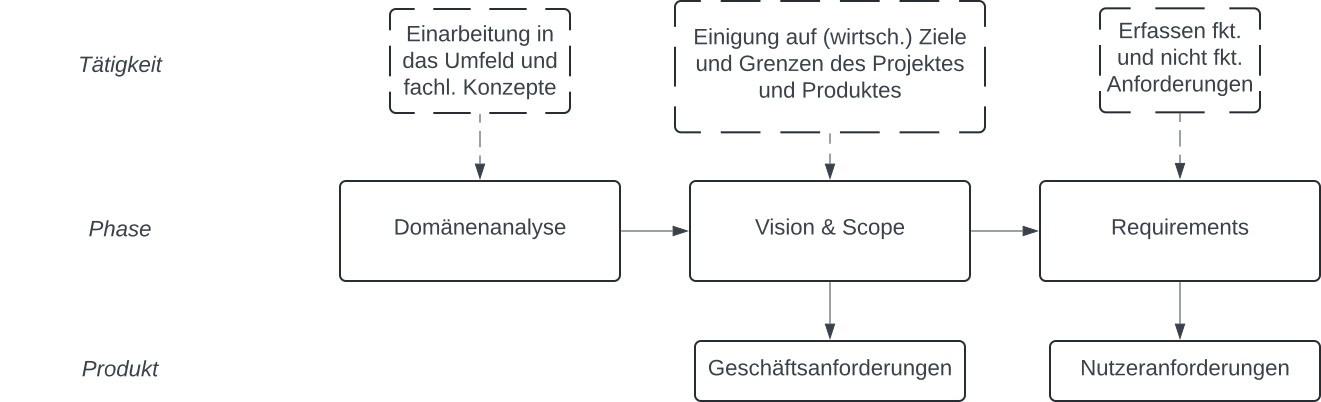
\includegraphics[scale=0.35]{chapters/Requirements Engineering/img/requirementsengineering}
    \caption{Phasen des Requirement Engineerings sowie deren Tätigkeiten und Ergebnisse. (Quelle: in Anlehnung an~\cite[84]{Wed09})}
    \label{fig:requirementsengineering}
\end{figure}

